\documentclass[
  11pt,
  letterpaper,
   addpoints,
   %answers
  ]{exam}

\usepackage[utf8]{inputenc}
\usepackage{../exercise-preamble}
\usepackage{float}
\usepackage{subcaption}
\usepackage{pgfplots}
\pgfplotsset{compat=1.18}
\usepgfplotslibrary{groupplots}
% TikZ libraries needed for `right=.. of ..` and coordinate math
\usetikzlibrary{positioning,calc,arrows,arrows.meta}

% Configuración de numeración de páginas
\makeatletter
\def\@oddfoot{\hfil Página \thepage \hfil}
\def\@evenfoot{\hfil Página \thepage \hfil}
\def\@oddhead{}
\def\@evenhead{}
\makeatother

\begin{document}

% Configuración del encabezado usando comandos de la clase exam
\pagestyle{headandfoot}
\extraheadheight{0.5in} % Baja el encabezado aumentando el espacio superior
\firstpageheader{\textit{Análisis de señales}}{}{EL3203}
\runningheader{\textit{Análisis de señales}}{}{EL3203}
\firstpagefooter{}{\thepage}{}
\runningfooter{}{\thepage}{}
\headrule % Línea debajo del encabezado

% Numeración de página
\pagenumbering{arabic}

% Portada
\begin{center}
    \vspace*{1cm}
    
    % Logo superior
    \includegraphics[width=0.5\textwidth]{../fcfm_die}
    
    \vspace{2cm}
    
    % Líneas decorativas superiores
    
\begin{tikzpicture}
        \draw[line width=2pt, black!70] (0,0) -- (10,0);
        \draw[line width=0.5pt, black!50] (0,0.2) -- (10,0.2);
    \end{tikzpicture}
    
    \vspace{1cm}
    
    % Título principal
    {\fontsize{28}{34}\selectfont\bfseries 
   Análisis de señales}
    
    \vspace{0.5cm}
    
    {\Large\textbf{EL3203}}
    
    \vspace{1cm}
    
    % Líneas decorativas inferiores
    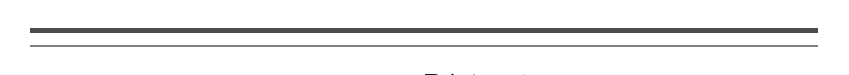
\begin{tikzpicture}
        \draw[line width=0.5pt, black!50] (0,0) -- (10,0);
        \draw[line width=2pt, black!70] (0,0.2) -- (10,0.2);
    \end{tikzpicture}
    
    \vspace{1.5cm}
    
    % Subtítulo
    {\LARGE\itshape Auxiliar 7 - Teorema del Muestreo}
    
    \vspace{0.5cm}
    {\large Prof Jorge Silva.}\\
    {\large Prof Auxiliar Erik Sáez Aravena.}
    
    % Decoración con símbolo matemático de fondo
    \begin{tikzpicture}[remember picture, overlay]
        \node[opacity=0.2, rotate=0] at ([yshift=-6cm]current page.center) {
            \scalebox{8}{$\mathcal{F}$}\color{black!10}
        };
    \end{tikzpicture}
    
    \vfill
    

    \vspace{1cm}
    
\end{center}

\newpage
%----------------------------
\section{Resumen}

\subsection*{1. Notación y Definiciones}
Algunas definiciones y notaciones clave para el análisis de señales muestreadas:
\textbf{Señales:}
\begin{itemize}
  \item $x_a(t)$: señal analógica (tiempo continuo)
  \item $x(n)$: señal discreta (tiempo discreto), obtenida muestreando $x_a(t)$
  \item Relación de muestreo: $x(n) = x_a(nT_s)$, donde $n \in \mathbb{Z}$
\end{itemize}

\textbf{Parámetros de muestreo:}
\begin{itemize}
  \item $T_s$: período de muestreo
  \item $F_s = T_s^{-1}$: frecuencia de muestreo
  \item $B$: ancho de banda de la señal (frecuencia máxima presente)
\end{itemize}

\textbf{Frecuencias:}
\begin{itemize}
  \item $F$: frecuencia continua (Hz)
  \item $f = \frac{F}{F_s}$: frecuencia normalizada (adimensional)
  \item $\omega = 2\pi f$: frecuencia angular normalizada (radianes)
\end{itemize}

\subsection*{2. Transformadas de Fourier}
Se definen las siguientes transformadas de Fourier para señales en tiempo continuo y discreto:
\textbf{Transformada de Fourier en tiempo continuo:}
\begin{align}
  X_a(F) &= \int_{-\infty}^{\infty} x_a(t)e^{-j2\pi Ft} dt \\
  x_a(t) &= \int_{-\infty}^{\infty} X_a(F)e^{j2\pi Ft} dF
\end{align}

\textbf{Transformada de Fourier en tiempo discreto:}
\begin{align}
  X(\omega) &= \sum_{n=-\infty}^{\infty} x(n)e^{-j\omega n} \\
  x(n) &= \frac{1}{2\pi} \int_{-\pi}^{\pi} X(\omega)e^{j\omega n} d\omega
\end{align}

Nota: $X(\omega)$ es periódica con período $2\pi$, o equivalentemente, $X(2\pi f)$ es periódica con período 1.

\subsection*{3. Teorema del Muestreo}

\textbf{Espectro de la señal muestreada:}

Cuando se muestrea una señal analógica $x_a(t)$ con frecuencia $F_s$, el espectro de la señal discreta resultante $x(n)$ está dado por:
\begin{equation}
  X(2\pi f) = F_s \sum_{k=-\infty}^{\infty} X_a(fF_s + kF_s) = F_s \sum_{k=-\infty}^{\infty} X_a(F + kF_s)
\end{equation}

donde $F = fF_s$ es la frecuencia continua.

\subsection*{4. Condición de Nyquist (Criterio de Muestreo)}

Para recuperar perfectamente la señal analógica original $x_a(t)$ a partir de sus muestras $x(n)$, debe cumplirse:
\begin{equation}
  \boxed{F_s \geq 2B} \quad \Leftrightarrow \quad \boxed{T_s \leq \frac{1}{2B}}
\end{equation}

donde $B$ es el ancho de banda de la señal (frecuencia máxima presente).

\textbf{Frecuencia de Nyquist:} $F_{\text{Nyquist}} = 2B$ es la frecuencia mínima de muestreo requerida.

\begin{itemize}
  \item Si $F_s \geq 2B$: No hay aliasing, las réplicas espectrales no se superponen, y el espectro se simplifica a:
  \begin{equation}
    X(2\pi f) = F_s X_a(fF_s), \quad f \in \left(-\frac{1}{2}, \frac{1}{2}\right]
  \end{equation}
  
  \item Si $F_s < 2B$: Hay \textbf{aliasing}, las réplicas espectrales se superponen, y la información original se pierde irreversiblemente.
\end{itemize}

\subsection*{5. Reconstrucción de la Señal (Fórmula de Interpolación de Shannon)}

Cuando se cumple la condición de Nyquist, la señal original puede reconstruirse perfectamente mediante:
\begin{equation}
  x_a(t) = \sum_{n=-\infty}^{\infty} x(n) \text{sinc}\left(\pi\frac{t - nT_s}{T_s}\right) = \sum_{n=-\infty}^{\infty} x_a(nT_s) \text{sinc}\left(\pi F_s(t - nT_s)\right)
\end{equation}

donde la función sinc normalizada se define como:
\begin{equation}
  \text{sinc}(\pi x) = \frac{\sin(\pi x)}{\pi x}
\end{equation}

\begin{itemize}
  \item Cada muestra $x(nT_s)$ contribuye con una función sinc centrada en $t = nT_s$
  \item Las funciones sinc tienen la propiedad de que $\text{sinc}(0) = 1$ y $\text{sinc}(n\pi) = 0$ para $n \neq 0$
  \item La reconstrucción es equivalente a pasar las muestras por un filtro pasa-bajos ideal con frecuencia de corte $F_s/2$
\end{itemize}

\subsection*{6. Recursos Interactivos}

Para una mejor comprensión visual del teorema del muestreo y sus implicaciones, se recomiendan los siguientes recursos interactivos:

\begin{itemize}
  \item \textbf{Interpolación y Muestreo:} \\
  \url{https://cs1230.graphics/demos/scaling/ip.html}
  
  \item \textbf{Visualización del Teorema del Muestreo:} \\
  \url{https://resources.nerdfirst.net/sampling.html}
\end{itemize}

Estos sitios permiten experimentar de forma interactiva con diferentes frecuencias de muestreo y observar en tiempo real los efectos del aliasing y la reconstrucción de señales.

\newpage

\begin{questions}

\question Sea $x_a(t)$ una señal analógica de banda limitada con transformada de Fourier $X_a(F)$ y período de muestreo $T_s = \frac{1}{F_s}$. Se define la señal discreta muestreada como $x(n) = x_a(nT_s)$ para $n \in \mathbb{Z}$.

\begin{parts}
  \part Demuestre que la transformada de Fourier discreta $X(\omega)$ de la señal muestreada puede escribirse en términos de la transformada continua como:
  \begin{equation}
    X(\omega) = \sum_{n=-\infty}^{\infty} x_a(nT_s)e^{-j\omega n}
  \end{equation}
  
  y que esta se relaciona con $X_a(F)$ mediante:
  \begin{equation}
    X(2\pi f) = F_s \sum_{k=-\infty}^{\infty} X_a(fF_s + kF_s)
  \end{equation}
  
  donde $f = \frac{F}{F_s}$ es la frecuencia normalizada.
  
  \begin{solution}
    
    La estrategia consiste en expresar la misma cantidad $x(n)$ de dos formas diferentes y luego igualarlas:
    \begin{itemize}
      \item Evaluación de la señal continua en puntos discretos (usando la transformada inversa continua)
      \item Usar la transformada inversa discreta (usando la transformada inversa discreta)
    \end{itemize}
    
    Al igualar ambas expresiones, podremos relacionar los espectros $X(2\pi f)$ y $X_a(F)$.
    
    
    Sabemos que la señal continua $x_a(t)$ puede recuperarse de su transformada de Fourier mediante:
    \begin{equation}
      x_a(t) = \int_{-\infty}^{\infty} X_a(F)e^{\left(j2\pi Ft\right)} dF
    \end{equation}
    
    Como $x(n) = x_a(nT_s)$, evaluamos la expresión anterior en $t = nT_s$ y usando $F_s = T_s^{-1}$:
    \begin{equation}
      x(n) = x_a(nT_s) = \int_{-\infty}^{\infty} X_a(F)e^{\left(j2\pi \frac{F}{F_s}n\right)} dF
    \end{equation}
    
    \textit{Nota: Aquí usamos la transformada continua porque $x_a(t)$ es una señal continua. Simplemente la evaluamos en puntos discretos.}
    
    Por otro lado, como $x(n)$ es una señal discreta, también puede expresarse mediante su transformada inversa de Fourier discreta:
    \begin{equation}
      x(n) = \int_{-\frac{1}{2}}^{\frac{1}{2}} X(2\pi f)e^{\left(j2\pi fn\right)} df
    \end{equation}
    
    \textit{Nota: Aquí usamos la transformada discreta porque $x(n)$ es una secuencia discreta con espectro periódico.}

    
    Como ambas expresiones representan el mismo valor $x(n)$, tenemos la siguiente identidad:
    \begin{equation}
      \int_{-\frac{1}{2}}^{\frac{1}{2}} X(2\pi f) e^{\left(j2\pi fn\right)} df = \int_{-\infty}^{\infty} X_a(F)e^{\left(j2\pi \frac{F}{F_s}n\right)} dF
    \end{equation}
    
    \textit{Observación importante: En el lado izquierdo tenemos una integral sobre frecuencias normalizadas $f \in [-1/2, 1/2]$ (dominio de la transformada discreta), mientras que en el lado derecho tenemos una integral sobre todas las frecuencias continuas $F \in (-\infty, \infty)$. Nuestro objetivo es manipular el lado derecho para expresarlo también como una integral sobre $[-1/2, 1/2]$.}
    
    Definimos la siguiente función indexada por $F$:
    \begin{equation}
      \Phi_F(n) = e^{\left(j2\pi \frac{F}{F_s}n\right)}
    \end{equation}
    
    Esta función tiene las siguientes propiedades de periodicidad:
    \begin{align}
      \Phi_{F+F_s}(n) &= e^{\left(j2\pi \frac{F+F_s}{F_s}n\right)} = e^{\left(j2\pi \frac{F}{F_s}n\right)} \cdot e^{\left(j2\pi n\right)} = \Phi_F(n) \quad \forall n \in \mathbb{Z}\\
      \Phi_{F+\ell F_s}(n) &= \Phi_F(n) \quad \forall n \in \mathbb{Z}, \forall \ell \in \mathbb{Z}
    \end{align}
    
    Por lo tanto, podemos descomponer la integral sobre toda la recta real como suma de integrales sobre intervalos de longitud $F_s$:
    \begin{equation}
      \int_{-\infty}^{\infty} X_a(F)\Phi_F(n) dF = \sum_{k \in \mathbb{Z}} \int_{-\frac{F_s}{2} + kF_s}^{\frac{F_s}{2} + kF_s} X_a(F)\Phi_F(n) dF
    \end{equation}
    
    Realizando el cambio de variable $\hat{F} = F - kF_s$ (entonces $dF = d\hat{F}$), tenemos:
    \begin{align}
      \int_{-\infty}^{\infty} X_a(F)\Phi_F(n) dF &= \sum_{k \in \mathbb{Z}} \int_{-\frac{F_s}{2}}^{\frac{F_s}{2}} X_a(\hat{F} + kF_s) \cdot \Phi_{\hat{F}+kF_s}(n) d\hat{F}\\
      &= \sum_{k \in \mathbb{Z}} \int_{-\frac{F_s}{2}}^{\frac{F_s}{2}} X_a(\hat{F} + kF_s) \cdot \Phi_{\hat{F}}(n) d\hat{F}\\
      &= \int_{-\frac{F_s}{2}}^{\frac{F_s}{2}} \left[\sum_{k \in \mathbb{Z}} X_a(\hat{F} + kF_s)\right] \cdot \Phi_{\hat{F}}(n) d\hat{F}\\
      &= \int_{-\frac{F_s}{2}}^{\frac{F_s}{2}} \left[\sum_{k \in \mathbb{Z}} X_a(\hat{F} + kF_s)\right] \cdot e^{\left(j2\pi \frac{\hat{F}}{F_s}n\right)} d\hat{F}
    \end{align}
    
    donde en el segundo paso usamos la propiedad de periodicidad $\Phi_{\hat{F}+kF_s}(n) = \Phi_{\hat{F}}(n)$. Ahora realizamos el cambio de variable $f = \frac{\hat{F}}{F_s}$ (frecuencia normalizada), por lo que $d\hat{F} = F_s df$:
    \begin{align}
      \int_{-\infty}^{\infty} X_a(F)\Phi_F(n) dF &= \int_{-\frac{1}{2}}^{\frac{1}{2}} \left[\sum_{k \in \mathbb{Z}} X_a(fF_s + kF_s)\right] \cdot e^{\left(j2\pi fn\right)} \cdot F_s df\\
      &= \int_{-\frac{1}{2}}^{\frac{1}{2}} F_s \left[\sum_{k \in \mathbb{Z}} X_a(fF_s + kF_s)\right] e^{\left(j2\pi fn\right)} df
    \end{align}
    
    Comparando con la identidad que establecimos en el Paso 3:
    \begin{equation}
      \int_{-\frac{1}{2}}^{\frac{1}{2}} X(2\pi f) e^{\left(j2\pi fn\right)} df = \int_{-\frac{1}{2}}^{\frac{1}{2}} F_s \left[\sum_{k \in \mathbb{Z}} X_a(fF_s + kF_s)\right] e^{\left(j2\pi fn\right)} df
    \end{equation}
    
    Como esta igualdad debe cumplirse para todo $n \in \mathbb{Z}$, y dado que las exponenciales complejas $\{e^{\left(j2\pi fn\right)}\}_{n \in \mathbb{Z}}$ forman una base ortogonal en el espacio de funciones periódicas, concluimos que los integrandos deben ser iguales:
    \begin{equation}
      \boxed{X(2\pi f) = F_s \sum_{k=-\infty}^{\infty} X_a(fF_s + kF_s)}
    \end{equation}
    
    para $f \in (-1/2, 1/2]$. Esta relación muestra que el espectro de la señal muestreada $X(2\pi f)$ es la suma de réplicas desplazadas del espectro continuo $X_a(F)$, escaladas por $F_s$. Cada réplica está centrada en $kF_s$ para $k \in \mathbb{Z}$. Esto explica el fenómeno de \textbf{aliasing} cuando las réplicas se superponen (cuando $F_s < 2B$).

  \end{solution}
  
  \part Para la señal anterior, demuestre que bajo la condición de muestreo de Nyquist ($F_s \geq 2B$, donde $B$ es el ancho de banda de la señal), la relación se simplifica a:
  \begin{equation}
    X(2\pi f) = F_s X_a(fF_s), \quad \text{para } f \in (-1/2, 1/2]
  \end{equation}
  
  y que por lo tanto es posible recuperar la señal original mediante:
  \begin{equation}
    x_a(t) = T_s \sum_{k \in \mathbb{Z}} x_a(kT_s) \text{sinc}\left(\pi\frac{t - kT_s}{T_s}\right)
  \end{equation}
  
  \begin{solution}
    Del resultado de la parte (a), tenemos:
    \begin{equation}
      X(2\pi f) = F_s\sum_{k=-\infty}^{\infty} X_a(fF_s + kF_s)
    \end{equation}
    
    Si la señal $x_a(t)$ es de banda limitada con ancho de banda $B$, entonces:
    \begin{equation}
      X_a(F) = 0 \quad \text{para } |F| > B
    \end{equation}
    
    
    Cuando se cumple la condición de Nyquist $F_s \geq 2B$, queremos demostrar que en la suma infinita:
    \begin{equation}
      X(2\pi f) = F_s \sum_{k=-\infty}^{\infty} X_a(fF_s + kF_s)
    \end{equation}
    solo sobrevive el término con $k=0$, es decir, que todos los demás términos son cero.

    
    Recordemos que $X_a(F) = 0$ para $|F| > B$ (señal de banda limitada). Por lo tanto, el término $X_a(fF_s + kF_s)$ solo es no nulo cuando:
    \begin{equation}
      |fF_s + kF_s| \leq B
    \end{equation}
    
    Es decir, cuando la frecuencia $fF_s + kF_s$ cae dentro de la banda de la señal original $[-B, B]$.Para $f \in (-1/2, 1/2]$, el producto $fF_s$ varía en:
    \begin{equation}
      -\frac{F_s}{2} < fF_s \leq \frac{F_s}{2}
    \end{equation}
    
    Por lo tanto, cuando sumamos $kF_s$, el término $k$-ésimo cubre el rango:
    \begin{equation}
      \underbrace{-\frac{F_s}{2} + kF_s}_{\text{límite inferior}} < fF_s + kF_s \leq \underbrace{\frac{F_s}{2} + kF_s}_{\text{límite superior}}
    \end{equation}
    
    Este es un intervalo de ancho $F_s$ centrado en $kF_s$. Ahora debemos analizar cuáles de estos intervalos se intersectan con la banda de la señal $[-B, B]$
    
    \textit{Caso $k = 0$:} El intervalo es $\left(-\frac{F_s}{2}, \frac{F_s}{2}\right]$. Como $F_s \geq 2B$, tenemos:
    \begin{equation}
      \frac{F_s}{2} \geq B \quad \Rightarrow \quad [-B, B] \subseteq \left(-\frac{F_s}{2}, \frac{F_s}{2}\right]
    \end{equation}
    Por lo tanto, este término SÍ contribuye para toda la banda de la señal.
    
    \textit{Caso $k = 1$:} El intervalo es $\left(\frac{F_s}{2}, \frac{3F_s}{2}\right]$. Para que haya intersección con $[-B, B]$, necesitaríamos:
    \begin{equation}
      \frac{F_s}{2} \leq B
    \end{equation}
    Pero bajo Nyquist, $\frac{F_s}{2} \geq B$, por lo que NO hay intersección. El intervalo está completamente a la derecha de $[-B, B]$.
    
    \textit{Caso $k = -1$:} El intervalo es $\left(-\frac{3F_s}{2}, -\frac{F_s}{2}\right]$. Para que haya intersección con $[-B, B]$, necesitaríamos:
    \begin{equation}
      -\frac{F_s}{2} \geq -B
    \end{equation}
    Pero bajo Nyquist, $-\frac{F_s}{2} \leq -B$, por lo que NO hay intersección. El intervalo está completamente a la izquierda de $[-B, B]$.
    
    \textit{Caso $k \neq 0, \pm 1$:} Estos intervalos están aún más alejados, por lo que tampoco hay intersección.
    
    Bajo la condición de Nyquist, solo el término $k=0$ contribuye, y todos los demás son cero:
    \begin{equation}
      \boxed{X(2\pi f) = F_s X_a(fF_s), \quad f \in (-1/2, 1/2]}
    \end{equation}
  
    \begin{itemize}
      \item La señal original ocupa $[-B, B]$
      \item La réplica $k=0$ cubre $\left(-\frac{F_s}{2}, \frac{F_s}{2}\right]$ y contiene completamente a $[-B, B]$
      \item Las réplicas $k=1$ y $k=-1$ cubren $\left(\frac{F_s}{2}, \frac{3F_s}{2}\right]$ y $\left(-\frac{3F_s}{2}, -\frac{F_s}{2}\right]$ respectivamente
      \item Como $\frac{F_s}{2} \geq B$, hay un "espacio de guarda" entre la banda de la señal y las réplicas adyacentes
      \item Este espacio de guarda evita el aliasing y permite la recuperación perfecta
    \end{itemize}
    
    
    Para recuperar $x_a(t)$, partimos de la transformada inversa de Fourier continua:
    \begin{equation}
      x_a(t) = \int_{-\infty}^{\infty} X_a(F)e^{\left(j2\pi Ft\right)} dF
    \end{equation}
    
    Dado que $X_a(F) = 0$ para $|F| > B$ y $B \leq F_s/2$ (condición de Nyquist), podemos limitar la integración:
    \begin{equation}
      x_a(t) = \int_{-\frac{F_s}{2}}^{\frac{F_s}{2}} X_a(F)e^{\left(j2\pi Ft\right)} dF
    \end{equation}
    
    Haciendo el cambio de variable $f = \frac{F}{F_s}$ (entonces $dF = F_s df$):
    \begin{equation}
      x_a(t) = \int_{-\frac{1}{2}}^{\frac{1}{2}} X_a(fF_s)e^{\left(j2\pi fF_s t\right)} F_s df
    \end{equation}
    
    Usando la relación simplificada $X_a(fF_s) = \frac{1}{F_s}X(2\pi f)$ obtenida bajo la condición de Nyquist:
    \begin{equation}
      x_a(t) = \int_{-\frac{1}{2}}^{\frac{1}{2}} \frac{1}{F_s}X(2\pi f)e^{\left(j2\pi fF_s t\right)} F_s df = \int_{-\frac{1}{2}}^{\frac{1}{2}} X(2\pi f)e^{\left(j2\pi fF_s t\right)} df
    \end{equation}
    
    De la parte (a), sabemos que la transformada de Fourier discreta está dada por:
    \begin{equation}
      X(2\pi f) = \sum_{n=-\infty}^{\infty} x(n)e^{\left(-j2\pi fn\right)} = \sum_{n=-\infty}^{\infty} x_a(nT_s)e^{\left(-j2\pi fn\right)}
    \end{equation}
    
    Sustituyendo esta expresión en la integral:
    \begin{align}
      x_a(t) &= \int_{-\frac{1}{2}}^{\frac{1}{2}} \left[\sum_{n=-\infty}^{\infty} x_a(nT_s)e^{\left(-j2\pi fn\right)}\right] e^{\left(j2\pi fF_s t\right)} df \\
      &= \sum_{n=-\infty}^{\infty} x_a(nT_s) \int_{-\frac{1}{2}}^{\frac{1}{2}} e^{\left(j2\pi f(F_s t - n)\right)} df
    \end{align}
    
    donde hemos intercambiado la suma y la integral (por convergencia uniforme).
    
    Calculando la integral:
    \begin{align}
      \int_{-\frac{1}{2}}^{\frac{1}{2}} e^{\left(j2\pi f(F_s t - n)\right)} df &= \frac{1}{j2\pi(F_s t - n)}\left[e^{\left(j\pi(F_s t - n)\right)} - e^{\left(-j\pi(F_s t - n)\right)}\right] \\
      &= \frac{1}{j2\pi(F_s t - n)} \cdot j2\sin(\pi(F_s t - n)) \\
      &= \frac{\sin(\pi(F_s t - n))}{\pi(F_s t - n)} \\
      &= \text{sinc}(\pi(F_s t - n))
    \end{align}
    
    Por lo tanto, sustituyendo en la expresión de $x_a(t)$:
    \begin{equation}
      x_a(t) = \sum_{n=-\infty}^{\infty} x_a(nT_s) \text{sinc}(\pi(F_s t - n))
    \end{equation}
    
    Usando $F_s = T_s^{-1}$, podemos reescribir $F_s t - n = \frac{t - nT_s}{T_s}$, por lo que:
    \begin{equation}
      x_a(t) = \sum_{n=-\infty}^{\infty} x_a(nT_s) \text{sinc}\left(\pi\frac{t - nT_s}{T_s}\right)
    \end{equation}
    
    Haciendo el cambio de índice $k = n$, obtenemos finalmente:
    \begin{equation}
      \boxed{x_a(t) = \sum_{k=-\infty}^{\infty} x_a(kT_s) \text{sinc}\left(\pi\frac{t - kT_s}{T_s}\right)}
    \end{equation}
    
    que también puede escribirse multiplicando y dividiendo por $T_s$:
    \begin{equation}
      x_a(t) = T_s \sum_{k=-\infty}^{\infty} x_a(kT_s) \text{sinc}\left(\pi\frac{t - kT_s}{T_s}\right)
    \end{equation}
    
    Esta es la fórmula de Shannon, que demuestra que bajo la condición de Nyquist, la señal analógica original puede reconstruirse perfectamente como una suma infinita de funciones sinc centradas en los instantes de muestreo, ponderadas por los valores de las muestras.
  \end{solution}
\end{parts}
%------------------------
  \question Considere una señal $x_a(t)$ con transformada de Fourier como se muestra en la figura
  
  \begin{figure}[H]
    \centering
    \begin{tikzpicture}
      \begin{axis}[
        axis lines=middle,
        xlabel={$F$},
        ylabel={$X_a(F)$},
        xmin=-2.5, xmax=2.5,
        ymin=-0.2, ymax=1.5,
        xtick={-2,-1,0,1,2},
        xticklabels={$-2F_0$,$-F_0$,$0$,$F_0$,$2F_0$},
        ytick={1},
        width=10cm,
        height=6cm,
      ]
      % Rectángulo izquierdo
      \addplot[thick, fill=black!20, pattern=north east lines] coordinates {
        (-2,0) (-2,1) (-1,1) (-1,0) (-2,0)
      };
      % Rectángulo derecho
      \addplot[thick, fill=black!20, pattern=north east lines] coordinates {
        (1,0) (1,1) (2,1) (2,0) (1,0)
      };
      \end{axis}
    \end{tikzpicture}
    \caption{Transformada de Fourier de la señal $x_a(t)$.}
  \end{figure}
  
  \begin{parts}
    \part Considere un proceso de muestreo donde $F_s = 4F_0$. Encuentre una expresión para $x(n)$. \textbf{Indicación:} Utilice la relación entre $X_a(F)$ y $X(2\pi f) = \text{DTFT}\{x(n)\}$ dadas por el teorema del muestreo.
    
    \begin{solution}
    
      Notemos que la señal $x(n)$ inducida por un muestreo con período $T_s$ está dada por:
      \begin{equation}
        x(n) = x_a(nT_s), \quad n \in \mathbb{Z}
      \end{equation}
      
      Además, sabemos que, por el teorema del muestreo (demostrado en la parte (a)), se cumple que el espectro de frecuencia de la señal muestreada $X(2\pi f)$ está dado por:
      \begin{equation}
        X(2\pi f) = \sum_{k \in \mathbb{Z}} F_s X_a(fF_s + kF_s),
      \end{equation}
      
      donde $F_s = T_s^{-1}$ es la frecuencia de muestreo. Notemos que, para la señal analógica original, a partir de la TF visual se puede ver que:
      \begin{equation}
        \text{supp}(X_a(f)) = [-2F_0, -F_0] \cup [F_0, 2F_0]
      \end{equation}
      Donde $\text{supp}(\cdot)$ denota el soporte de la función, es decir el conjunto donde la función es no nula.
  
      
      Para la $k$-ésima banda, la TF discreta está dada por $X_a(fF_s + kF_s)$, por lo que podemos calcular el soporte de cada banda y analizar cuáles de ellas tienen intersección con el intervalo fundamental $(-1/2, 1/2]$, de modo que aquellas bandas cuya intersección es nula pueden ser omitidas de la sumatoria. 
      
      Para calcular el soporte, debemos obtener los valores de frecuencia $f_k^{\text{low}}$ y $f_k^{\text{high}}$ que entregan los límites inferiores y superiores, respectivamente, del soporte de la señal analógica. Haciendo esto, notemos que estos deben ser tales que:
      \begin{equation}
        f_k^{\text{low}}F_s + kF_s = -2F_0 \quad \land \quad f_k^{\text{high}}F_s + kF_s = 2F_0
      \end{equation}
      
      Calculando cada uno, considerando que $F_s = 4F_0$, tenemos:
      \begin{align}
        f_k^{\text{low}}F_s + kF_s &= -2F_0 \\
        \Leftrightarrow 4f_k^{\text{low}}F_0 + 4kF_0 &= -2F_0 \\
        \Leftrightarrow 4f_k^{\text{low}} + 4k &= -2 \\
        \Leftrightarrow f_k^{\text{low}} &= -\frac{1}{2} - k
      \end{align}
      
      Para la frecuencia superior, haciendo un análisis similar se puede ver que $f_k^{\text{high}} = \frac{1}{2} - k$, por lo que:
      \begin{equation}
        \text{supp}(X_a(fF_s + kF_s)) = \left(-\frac{1}{2} - k, \frac{1}{2} - k\right]
      \end{equation}
      
      
      La expresión del soporte nos dice que para la banda $k$-ésima, el intervalo de frecuencias normalizadas $f$ que corresponde al soporte original de $X_a$ es $\left(-\frac{1}{2} - k, \frac{1}{2} - k\right]$. Esto se deriva de la transformación inversa:
      \begin{itemize}
        \item Soporte original de $X_a(F)$: $F \in [-2F_0, -F_0] \cup [F_0, 2F_0]$
        \item Para la banda $k$, buscamos valores de $f$ tales que $fF_s + kF_s$ caiga en este soporte
        \item Resolviendo: $-2F_0 \leq fF_s + kF_s \leq 2F_0$ y usando $F_s = 4F_0$, obtenemos el intervalo desplazado
      \end{itemize}
      
      Evaluando para valores específicos de $k$:
      \begin{align*}
        k = 0 &: \quad \text{supp} = \left(-\frac{1}{2} - 0, \frac{1}{2} - 0\right] = \left(-\frac{1}{2}, \frac{1}{2}\right] \\[0.2cm]
        k = 1 &: \quad \text{supp} = \left(-\frac{1}{2} - 1, \frac{1}{2} - 1\right] = \left(-\frac{3}{2}, -\frac{1}{2}\right] \\[0.2cm]
        k = -1 &: \quad \text{supp} = \left(-\frac{1}{2} - (-1), \frac{1}{2} - (-1)\right] = \left(\frac{1}{2}, \frac{3}{2}\right] \\[0.2cm]
        k = 2 &: \quad \text{supp} = \left(-\frac{1}{2} - 2, \frac{1}{2} - 2\right] = \left(-\frac{5}{2}, -\frac{3}{2}\right] \\[0.2cm]
        k = -2 &: \quad \text{supp} = \left(-\frac{1}{2} + 2, \frac{1}{2} + 2\right] = \left(\frac{3}{2}, \frac{5}{2}\right]
      \end{align*}
      
      Ahora debemos determinar cuáles de estas bandas intersectan el intervalo fundamental $(-1/2, 1/2]$. Esto \textbf{no es una imposición}, sino una \textbf{consecuencia geométrica} de analizar cada caso:
      
      \begin{itemize}
        \item \textbf{Para $k=0$:} El soporte es $\left(-\frac{1}{2}, \frac{1}{2}\right]$, que es exactamente el intervalo fundamental. Por lo tanto, \textbf{sí hay intersección completa} y esta banda contribuye a la suma.
        
        \item \textbf{Para $k=1$:} El soporte es $\left(-\frac{3}{2}, -\frac{1}{2}\right]$. Este intervalo está completamente a la \textit{izquierda} del intervalo fundamental $(-1/2, 1/2]$, por lo que \textbf{no hay intersección}. Matemáticamente: $\left(-\frac{3}{2}, -\frac{1}{2}\right] \cap \left(-\frac{1}{2}, \frac{1}{2}\right] = \emptyset$.
        
        \item \textbf{Para $k=-1$:} El soporte es $\left(\frac{1}{2}, \frac{3}{2}\right]$. Este intervalo está completamente a la \textit{derecha} del intervalo fundamental $(-1/2, 1/2]$, por lo que \textbf{no hay intersección}. Matemáticamente: $\left(\frac{1}{2}, \frac{3}{2}\right] \cap \left(-\frac{1}{2}, \frac{1}{2}\right] = \emptyset$.
        
        \item \textbf{Para $|k| \geq 2$:} Los soportes están aún más alejados del intervalo fundamental, por lo que tampoco hay intersección.
      \end{itemize}
      
      Como resultado de este análisis geométrico, todos los términos con $k \neq 0$ en la suma son idénticamente cero en el intervalo $f \in (-1/2, 1/2]$, porque sus soportes no intersectan este intervalo. Por lo tanto, la TF de la señal muestreada se simplifica a:
      \begin{equation}
        X(2\pi f) = F_s X_a(fF_s) = 4F_0 X_a(4fF_0)
      \end{equation}
      
      \begin{figure}[H]
        \centering
        \begin{tikzpicture}
          \begin{axis}[
            axis lines=middle,
            xlabel={$f$},
            ylabel={$X(2\pi f)$},
            xmin=-0.6, xmax=0.6,
            ymin=-0.2, ymax=5,
            xtick={-0.5,-0.25,0,0.25,0.5},
            xticklabels={$-\frac{1}{2}$,$-\frac{1}{4}$,$0$,$\frac{1}{4}$,$\frac{1}{2}$},
            ytick={4},
            yticklabels={$4F_0$},
            width=12cm,
            height=6cm,
          ]
          % Rectángulo izquierdo
          \addplot[thick, fill=blue!20, pattern=north east lines, pattern color=blue] coordinates {
            (-0.5,0) (-0.5,4) (-0.25,4) (-0.25,0) (-0.5,0)
          };
          % Rectángulo derecho
          \addplot[thick, fill=blue!20, pattern=north east lines, pattern color=blue] coordinates {
            (0.25,0) (0.25,4) (0.5,4) (0.5,0) (0.25,0)
          };
          \end{axis}
        \end{tikzpicture}
        \caption{Espectro de la señal muestreada $X(2\pi f)$ para $F_s = 4F_0$ (sin aliasing).}
      \end{figure}
      
      
      Para determinar los intervalos exactos donde $X(2\pi f) \neq 0$, debemos mapear el soporte original de $X_a(F)$ al dominio de frecuencia normalizada $f$. Recordemos que la relación es:
      \begin{equation}
        X(2\pi f) = F_s X_a(fF_s) = 4F_0 X_a(4fF_0)
      \end{equation}
      
      El soporte original de $X_a(F)$ es $[-2F_0, -F_0] \cup [F_0, 2F_0]$. Para encontrar el soporte en términos de $f$, resolvemos:
      
      \begin{itemize}
        \item \textbf{Banda izquierda:} $X_a(F) \neq 0$ para $F \in [-2F_0, -F_0]$. Sustituyendo $F = 4fF_0$:
        \begin{align}
          -2F_0 &\leq 4fF_0 \leq -F_0 \\
          -2 &\leq 4f \leq -1 \\
          -\frac{1}{2} &\leq f \leq -\frac{1}{4}
        \end{align}
        Por lo tanto, $X(2\pi f) = 4F_0$ para $f \in \left[-\frac{1}{2}, -\frac{1}{4}\right]$.
        
        \item \textbf{Banda derecha:} $X_a(F) \neq 0$ para $F \in [F_0, 2F_0]$. Sustituyendo $F = 4fF_0$:
        \begin{align}
          F_0 &\leq 4fF_0 \leq 2F_0 \\
          1 &\leq 4f \leq 2 \\
          \frac{1}{4} &\leq f \leq \frac{1}{2}
        \end{align}
        Por lo tanto, $X(2\pi f) = 4F_0$ para $f \in \left[\frac{1}{4}, \frac{1}{2}\right]$.
        
        \item \textbf{Región central:} Para $f \in \left(-\frac{1}{4}, \frac{1}{4}\right)$, tenemos $4fF_0 \in (-F_0, F_0)$, que está fuera del soporte de $X_a(F)$, por lo que $X(2\pi f) = 0$.
      \end{itemize}
      
      Por lo tanto, la expresión completa del espectro discreto es:
      \begin{equation}
        X(2\pi f) = \begin{cases}
          4F_0 & \text{si } f \in (-1/2, -1/4] \\
          0 & \text{si } f \in (-1/4, 1/4] \\
          4F_0 & \text{si } f \in (1/4, 1/2]
        \end{cases}
      \end{equation}
  
      Luego, podemos aplicar la inversa de Fourier para obtener la señal en el dominio del tiempo, de lo que tenemos:
      \begin{align}
        x(n) &= \int_{-1/2}^{1/2} X(2\pi f)e^{\left(j2\pi fn\right)} df \\
        &= 4F_0 \int_{-1/2}^{-1/4} e^{\left(j2\pi fn\right)} df + 4F_0 \int_{1/4}^{1/2} e^{\left(j2\pi fn\right)} df \\
        &= \frac{4F_0}{j2\pi n} \left[e^{\left(-j\frac{\pi}{2}n\right)} - e^{\left(-j\pi n\right)} + e^{\left(j\pi n\right)} - e^{\left(j\frac{\pi}{2}n\right)}\right]
      \end{align}
      
      Notemos que las exponenciales se pueden agrupar, considerando que:
      \begin{equation}
        \sin(\theta) = \frac{e^{\left(j\theta\right)} - e^{\left(-j\theta\right)}}{j2}
      \end{equation}
      
      por lo que tenemos:
      \begin{equation}
        x(n) = \frac{4F_0}{j2\pi n} \left[j2\sin(\pi n) - j2\sin\left(\frac{\pi}{2}n\right)\right] = \frac{4F_0}{\pi n} \left[\sin(\pi n) - \sin\left(\frac{\pi}{2}n\right)\right]
      \end{equation}
      
      Luego, notemos que, dado que $n \in \mathbb{Z}$, se tiene $\sin(\pi n) = 0$, por lo que ese término no se considera dentro de la expresión. Así, finalmente tenemos que la señal muestreada está dada por:
      \begin{equation}
        \boxed{x(n) = -4F_0 \frac{\sin\left(\frac{\pi}{2}n\right)}{\pi n}}
      \end{equation}
      
      Notemos además que, considerando la función sinc la cual está definida como:
      \begin{equation}
        \text{sinc}(\pi x) = \frac{\sin(\pi x)}{\pi x}
      \end{equation}
      
      podemos escribir la señal en términos de esta función como:
      \begin{equation}
        x(n) = -2F_0 \text{sinc}\left(\frac{\pi}{2}n\right)
      \end{equation}
    \end{solution}
    
    \part Repita el análisis del punto anterior si $F_s = 3F_0$ y comente si es posible recuperar $x_a(t)$ a partir de $x(n)$
    
    \begin{solution}
  
      El procedimiento a seguir para este caso es análogo al usado para la frecuencia anterior. En este caso, notemos que para la $k$-ésima banda las frecuencias máximas y mínimas son:
      \begin{align}
        3f_k^{\text{low}}F_0 + 3kF_0 &= -2F_0 \\
        \Leftrightarrow 3f_k^{\text{low}} + 3k &= -2 \\
        \Leftrightarrow f_k^{\text{low}} &= -\frac{2}{3} - k
      \end{align}
      
      \begin{align}
        3f_k^{\text{high}}F_0 + 3kF_0 &= 2F_0 \\
        \Leftrightarrow 3f_k^{\text{high}} + 3k &= 2 \\
        \Leftrightarrow f_k^{\text{high}} &= \frac{2}{3} - k
      \end{align}
      
      por lo que el soporte de la $k$-ésima banda es:
      \begin{equation}
        \text{supp}(X_a(3fF_0 + 3kF_0)) = \left(-\frac{2}{3} - k, \frac{2}{3} - k\right]
      \end{equation}
      
      En este caso, a diferencia del caso anterior, notemos que las bandas $k = 1$ y $k = -1$ \textbf{sí intersectan} al intervalo fundamental, ya que los soportes de estas dos bandas son $(-5/3, -1/3]$ y $(1/3, 5/3]$, respectivamente. Esto significa que, ahora, al reconstruir el espectro discreto debemos considerar estos dos términos en la sumatoria, por lo que tenemos:
      \begin{equation}
        X(2\pi f) = 3F_0 [X_a(3fF_0 - 3F_0) + X_a(3fF_0) + X_a(3fF_0 + 3F_0)]
      \end{equation}
      
      \begin{figure}[H]
        \centering
        \begin{tikzpicture}
          \begin{axis}[
            axis lines=middle,
            xlabel={$f$ },
            ylabel={$X(2\pi f)$},
            xmin=-0.6, xmax=0.6,
            ymin=-0.2, ymax=7,
            xtick={-0.5,-0.333,0,0.333,0.5},
            xticklabels={$-\frac{1}{2}$,$-\frac{1}{3}$,$0$,$\frac{1}{3}$,$\frac{1}{2}$},
            ytick={3,6},
            yticklabels={$3F_0$,$6F_0$},
            width=12cm,
            height=6cm,
          ]
          % Banda k=-1 (roja, parcialmente fuera)
          \addplot[thick, fill=red!20, pattern=dots, pattern color=red, opacity=0.7] coordinates {
            (-0.6,0) (-0.6,3) (-0.333,3) (-0.333,0) (-0.6,0)
          };
          \node[red] at (axis cs:-0.47,3.5) {\small $k=-1$};
          
          % Banda k=0 (azul, central)
          \addplot[thick, fill=blue!20, pattern=north east lines, pattern color=blue, opacity=0.7] coordinates {
            (-0.5,0) (-0.5,3) (-0.333,3) (-0.333,0) (-0.5,0)
          };
          \addplot[thick, fill=blue!20, pattern=north east lines, pattern color=blue, opacity=0.7] coordinates {
            (0.333,0) (0.333,3) (0.5,3) (0.5,0) (0.333,0)
          };
          \node[blue] at (axis cs:0,3.5) {\small $k=0$};
          
          % Banda k=1 (verde, parcialmente fuera)
          \addplot[thick, fill=green!30, pattern=dots, pattern color=green!70!black, opacity=0.7] coordinates {
            (0.333,0) (0.333,3) (0.6,3) (0.6,0) (0.333,0)
          };
          \node[green!70!black] at (axis cs:0.47,3.5) {\small $k=1$};
          
          % Superposición (aliasing) - regiones con doble altura
          \addplot[thick, fill=orange!40, pattern=crosshatch, pattern color=orange!70!red] coordinates {
            (-0.5,3) (-0.5,6) (-0.333,6) (-0.333,3) (-0.5,3)
          };
          \addplot[thick, fill=orange!40, pattern=crosshatch, pattern color=orange!70!red] coordinates {
            (0.333,3) (0.333,6) (0.5,6) (0.5,3) (0.333,3)
          };
          
          % Marcadores de aliasing
          \node[orange!70!red, font=\scriptsize] at (axis cs:-0.417,5) {Aliasing};
          \node[orange!70!red, font=\scriptsize] at (axis cs:0.417,5) {Aliasing};
          
          \end{axis}
        \end{tikzpicture}
        \caption{Espectro de la señal muestreada $X(2\pi f)$ para $F_s = 3F_0$ mostrando el aliasing. Las regiones naranjas indican la superposición de bandas.}
      \end{figure}
      
      Al escribir este espectro considerando la representación gráfica de $X_a(f)$, tenemos:
      \begin{equation}
        X(2\pi f) = \begin{cases}
          6F_0 & \text{si } f \in \left(-\frac{1}{2}, -\frac{1}{3}\right] \\[0.3cm]
          0 & \text{si } f \in \left(-\frac{1}{3}, \frac{1}{3}\right] \\[0.3cm]
          6F_0 & \text{si } f \in \left(\frac{1}{3}, \frac{1}{2}\right]
        \end{cases}
      \end{equation}
      
      donde notemos que se tiene $6F_0$ en vez de $3F_0$ ya que, a diferencia de la señal anterior, en este caso las componentes de las bandas adyacentes se superponen, haciendo que tengan una mayor amplitud.
      
      
      Luego, podemos aplicar la inversa de Fourier al igual que hicimos con la señal anterior, de donde tenemos:
      \begin{align}
        x(n) &= \int_{-1/2}^{1/2} X(2\pi f)e^{\left(j2\pi fn\right)} df \\
        &= 6F_0 \left[\int_{-1/2}^{-1/3} e^{\left(j2\pi fn\right)} df + \int_{1/3}^{1/2} e^{\left(j2\pi fn\right)} df\right] \\
        &= \frac{6F_0}{j2\pi n} \left[e^{\left(-j\frac{2\pi}{3}n\right)} - e^{\left(-j\pi n\right)} + e^{\left(j\pi n\right)} - e^{\left(j\frac{2\pi}{3}n\right)}\right]
      \end{align}
      
      Al igual que antes, podemos agrupar términos para formar sinusoidales, de donde tenemos:
      \begin{align}
        x(n) &= \frac{6F_0}{j2\pi n} \left[j2\sin(\pi n) - j2\sin\left(\frac{2\pi}{3}n\right)\right] \\
        &= -6F_0 \frac{\sin\left(\frac{2\pi}{3}n\right)}{\pi n},
      \end{align}
      
      donde, al igual que en la señal anterior, se tiene $\sin(\pi n) = 0$. Por lo tanto:
      \begin{equation}
        \boxed{x(n) = -6F_0 \frac{\sin\left(\frac{2\pi}{3}n\right)}{\pi n}}
      \end{equation}
      
      Además, análogo al caso anterior, esta señal puede ser escrita usando la función sinc como:
      \begin{equation}
        x(n) = -4F_0 \text{sinc}\left(\frac{2\pi}{3}n\right)
      \end{equation}
      
      
      \textit{No es posible recuperar $x_a(t)$ a partir de $x(n)$ cuando $F_s = 3F_0$}, ya que hay \textbf{aliasing}. Las componentes de las bandas $k=1$ y $k=-1$ se superponen con la banda fundamental en los intervalos $(-1/2, -1/3]$ y $(1/3, 1/2]$ respectivamente, lo cual no cumple la condición de Nyquist para evitar el aliasing.
      \begin{equation}
        F_s \geq 2B
      \end{equation}
      
      donde $B = 2F_0$ es el ancho de banda máximo de la señal (frecuencia máxima presente). En este caso:
      \begin{equation}
        F_s = 3F_0 < 4F_0 = 2B
      \end{equation}
      
      Por lo tanto, la condición de Nyquist \textbf{no se cumple} y la información original se pierde debido a la superposición espectral (aliasing).
    \end{solution}
  \end{parts}
%-----------------------


\end{questions}
\end{document}